% Chapter 8: Morphological Similarity, Convergence and Divergence

\section{Turning Profiles into Relations}

Two disciplines are morphologically similar when their embedding-space metric profiles are close after robust standardization. This is not document-level semantic similarity: two fields can be morphologically close without studying the same topics, using the same vocabulary, citing the same work, or belonging to the same institutional tradition. Their paper distributions have similar structural shape under the reduced metric representation.

Static similarity uses the full eleven-metric core from Chapter~5. For each metric, values are centered by the cross-subfield median and scaled by the interquartile range; field and domain profiles are averages of the robust-scaled subfield profiles. The primary distance used below is Euclidean distance between these standardized profiles, because it preserves magnitude differences in dispersion, local density, hubness, spectral structure, and full-period temporal indicators.

Temporal convergence and divergence use the eight structural metrics recomputed inside each five-year window. The three full-period temporal indicators are excluded from windowed pairwise distances because they are already summaries over time. Operationally, convergence means that the distance between two windowed profiles decreases from 2000--2004 to 2020--2024; divergence means that it increases.

\section{Static Similarity Across Disciplines}

The static field-level distance matrix gives a compact view of profile-space structure. If OpenAlex domains fully aligned with morphology, the diagonal domain blocks would be uniformly light and the off-block regions uniformly dark. Figure~\ref{fig:field_static_distance_heatmap} shows a weaker pattern. Some domain blocks are internally coherent, but many nearest profile-space relations cross domain boundaries.

\begin{figure}[H]
\centering
\caption[Pairwise field morphological distances]{Pairwise morphological distance between fields. Distances are computed from robust-scaled eleven-metric profiles; lower values indicate more similar morphology.}
\label{fig:field_static_distance_heatmap}
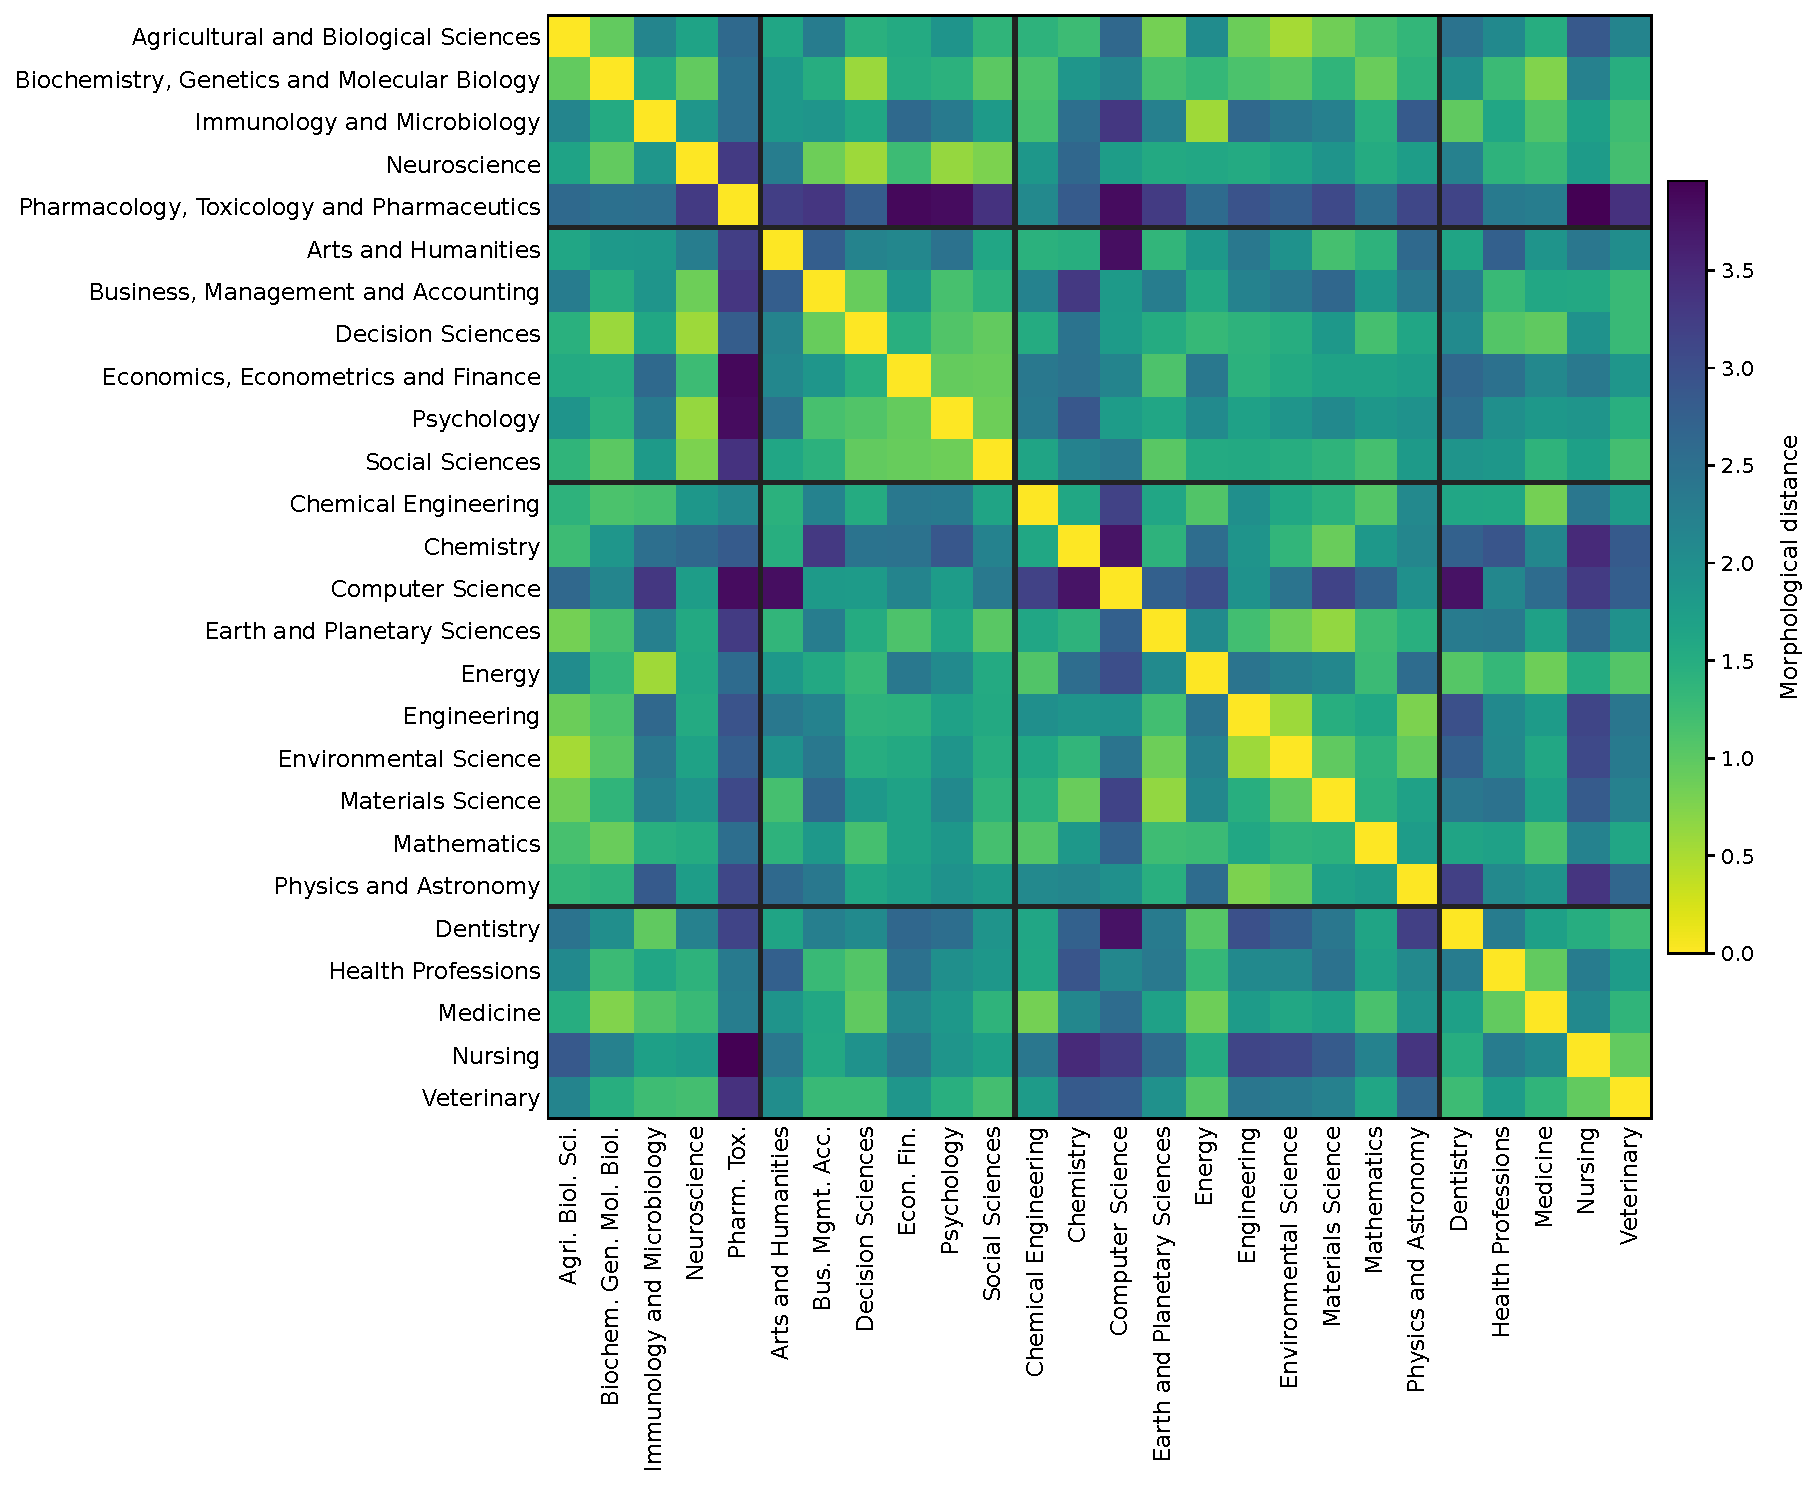
\includegraphics[width=\textwidth]{figures/fig_08_field_static_distance_heatmap.pdf}
\end{figure}

The closest Euclidean field pairs are not simply within-domain neighbors. Biochemistry, Genetics and Molecular Biology is closest to Medicine; Neuroscience is closest to Psychology; Chemical Engineering is close to Medicine; and Agricultural and Biological Sciences is close to Materials Science. These links do not imply shared content. They mean that the fields have similar standardized levels of compactness, dispersion, hubness, spectral structure, and temporal indicators. The comparison makes shape relations visible without turning them into topic relations.

Figure~\ref{fig:domain_pair_distance_structure} replaces the binary within--cross contrast with a domain-pair view. Within-domain field pairs have a lower overall median distance than cross-domain pairs, \(1.90\) versus \(2.20\), but the domain cells show where that average comes from. Social Sciences are the most internally coherent domain, while the closest cross-domain relation is between Life Sciences and Health Sciences. At field level, 18 of 26 fields have their nearest morphological neighbor outside their own domain. This is the chapter's clearest evidence that formal domains and morphology do not give the same structure.

\begin{figure}[H]
\centering
\caption[Domain-pair morphological distance structure]{Domain-pair morphological distance structure. Panel A reports median field-pair distances for each pair of OpenAlex domains; Panel B counts fields whose nearest morphological neighbor lies inside or outside their own domain.}
\label{fig:domain_pair_distance_structure}
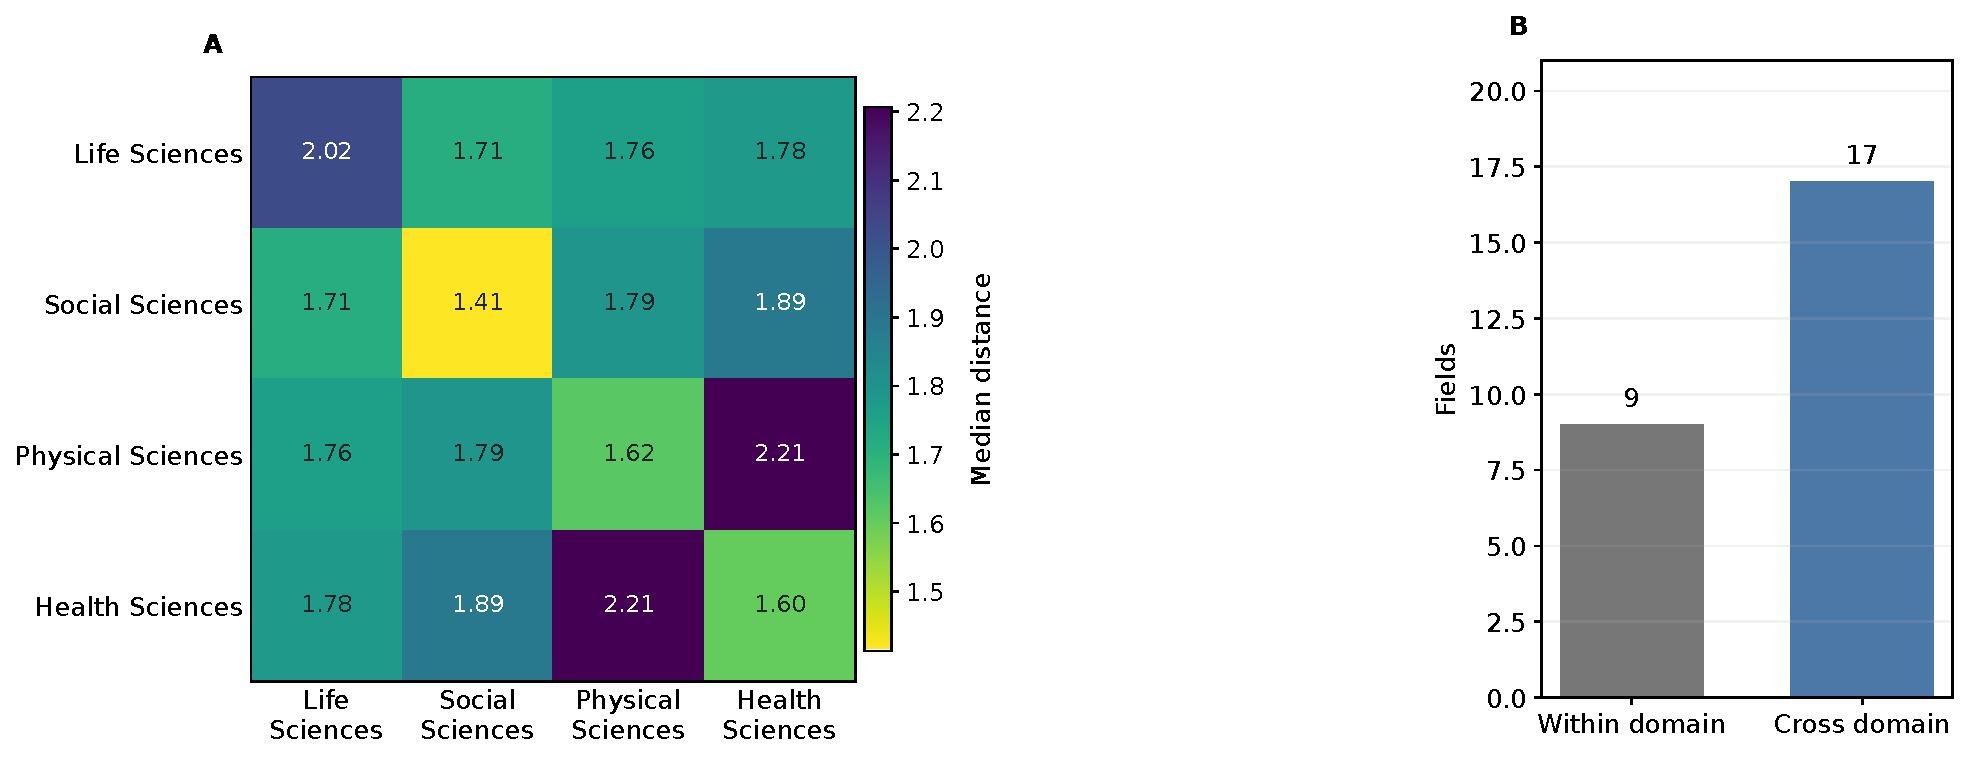
\includegraphics[width=\textwidth]{figures/fig_08_domain_pair_distance_structure.pdf}
\end{figure}

Figure~\ref{fig:field_nearest_neighbor_ring} makes the same result more concrete by turning the distance matrix into a directed nearest-neighbor map. Each arrow starts in a field and points to the field with the closest full-period morphology profile; dark arrows cross OpenAlex domain boundaries and grey arrows remain inside the same domain. The circular layout preserves domain membership, so the figure should be read as a stress test of the taxonomy: if domain labels fully organized morphology, most arrows would stay within their own sector.

\begin{figure}[H]
\centering
\caption[Directed field nearest-neighbor map]{Directed nearest-neighbor map between fields in morphology-profile space. Arrows point from each field to its nearest morphological neighbor under the robust-scaled eleven-metric distance; dark arrows indicate cross-domain nearest neighbors and grey arrows indicate within-domain nearest neighbors. Node size is proportional to the number of included subfields.}
\label{fig:field_nearest_neighbor_ring}
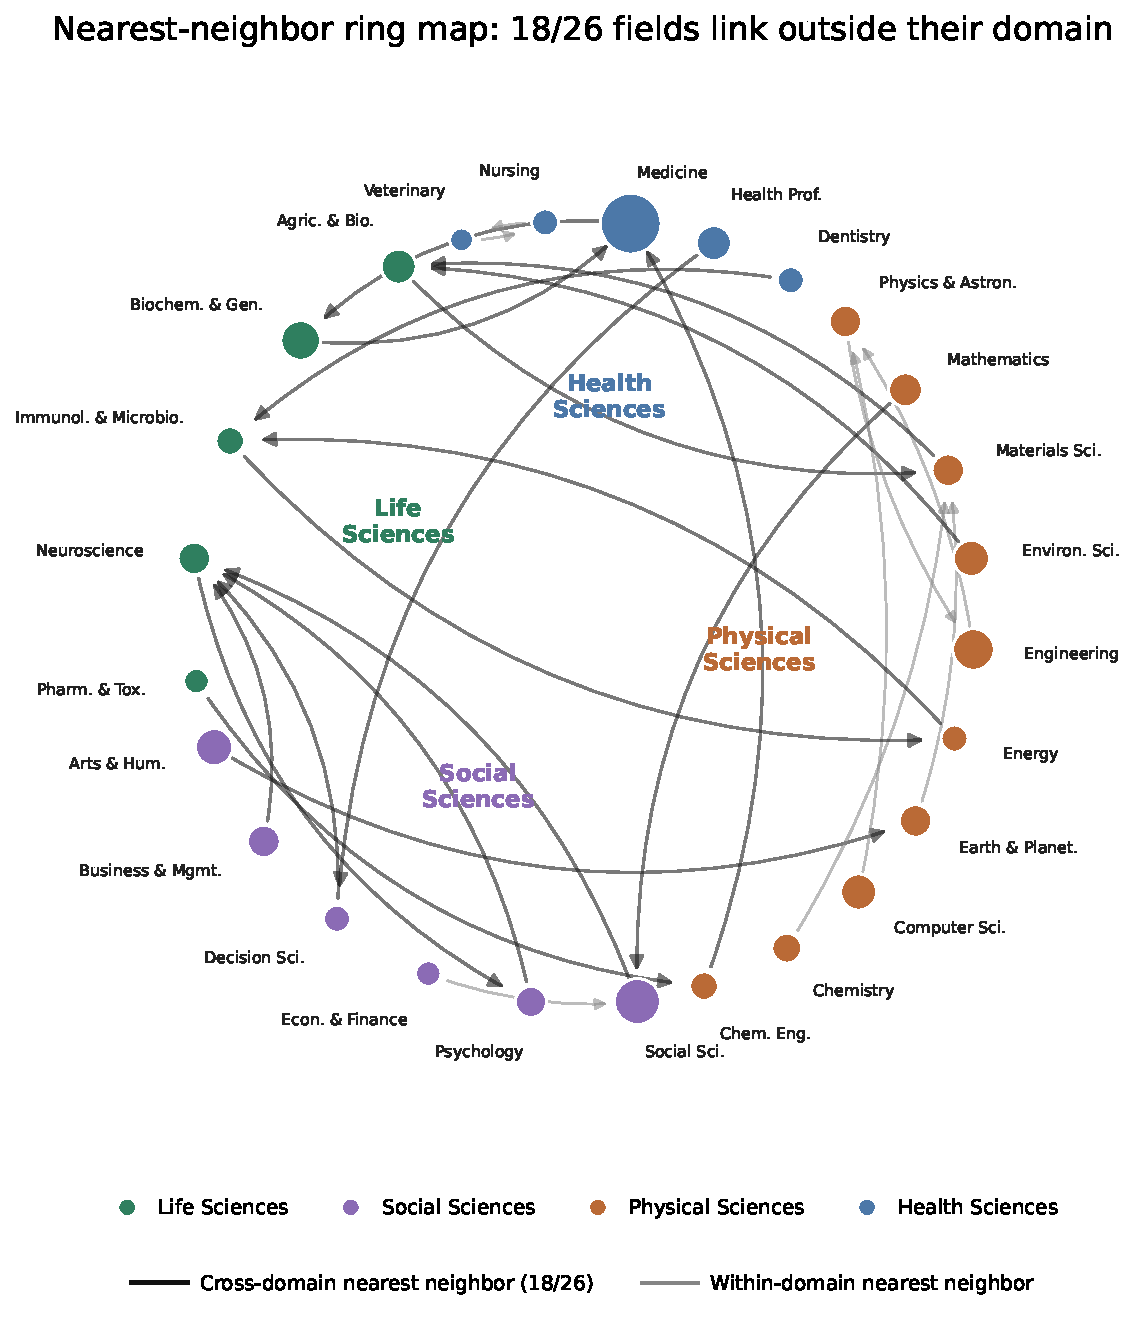
\includegraphics[width=\textwidth]{figures/fig_08_field_neighbor_variant_02_domain_ring.pdf}
\end{figure}

The map clarifies three aspects that are harder to see in the heatmap. First, cross-domain similarity is not a marginal exception but the dominant local relation: the dark chords are spread around the ring rather than concentrated in a single anomalous block. Second, several relations are reciprocal, including Medicine with Biochemistry, Genetics and Molecular Biology, Neuroscience with Psychology, Energy with Immunology and Microbiology, and Nursing with Veterinary. These reciprocal links identify local morphological pairs, not merely one-sided approximations. Third, some fields act as attractors for multiple neighbors. Materials Science receives links from Agricultural and Biological Sciences, Chemistry, and Earth and Planetary Sciences, while Neuroscience receives links from Business, Management and Accounting, Decision Sciences, and Social Sciences. The interpretation is therefore not that domains are irrelevant, but that domain membership is an incomplete predictor of field shape: morphology produces local affinities, bridges, and asymmetric pulls that the domain-level taxonomy smooths over.

\section{Convergence and Divergence Over Time}

The temporal picture is not global convergence. Across all 325 field pairs, mean Euclidean distance rises from \(1.44\) in 2000--2004 to \(1.81\) in 2020--2024. The same upward movement appears within domains, from \(1.39\) to \(1.70\), and across domains, from \(1.46\) to \(1.85\). Field-level morphology space becomes more separated on average, even though many individual pairs move closer. This supports the main argument because it separates average differentiation from selective convergence.

\begin{figure}[H]
\centering
\caption[Temporal field-pair distance trajectories]{Mean field-pair morphological distance across five-year windows using the eight windowed structural metrics.}
\label{fig:temporal_distance_trajectories}
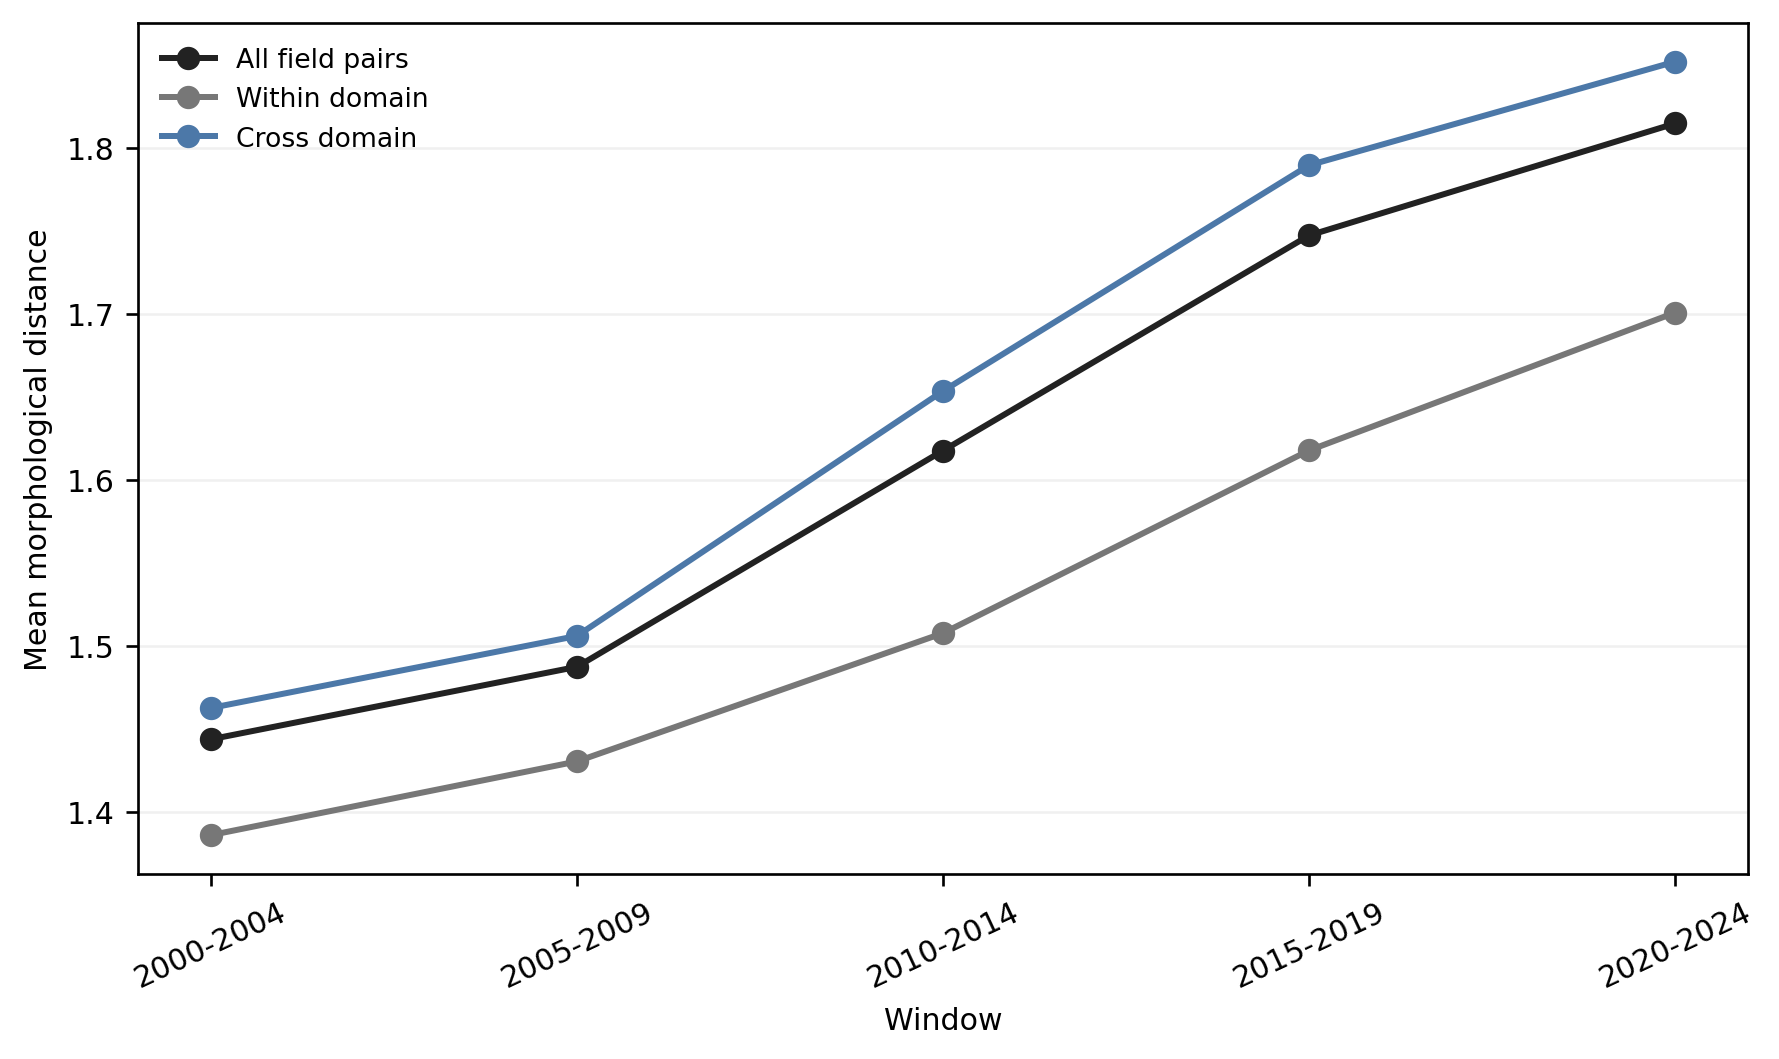
\includegraphics[width=0.88\textwidth]{figures/fig_08_temporal_distance_trajectories.png}
\end{figure}

This average expansion coexists with selective convergence: 97 field pairs decrease in distance, while 228 increase. The strongest convergences tend to involve shared declines in local distance and spectral dimensionality. Materials Science and Mathematics move from \(1.75\) to \(0.85\); Decision Sciences and Environmental Science from \(1.67\) to \(0.82\); and Economics, Econometrics and Finance and Psychology from \(1.53\) to \(0.70\). These are relative movements in metric-profile space, not evidence of intellectual merger.

\begin{figure}[H]
\centering
\caption[Strongest field convergence and divergence]{Strongest field-level convergence and divergence under Euclidean profile distance. Open markers are initial distances and filled markers are final distances; labels show final-minus-initial change.}
\label{fig:field_convergence_divergence_pairs}
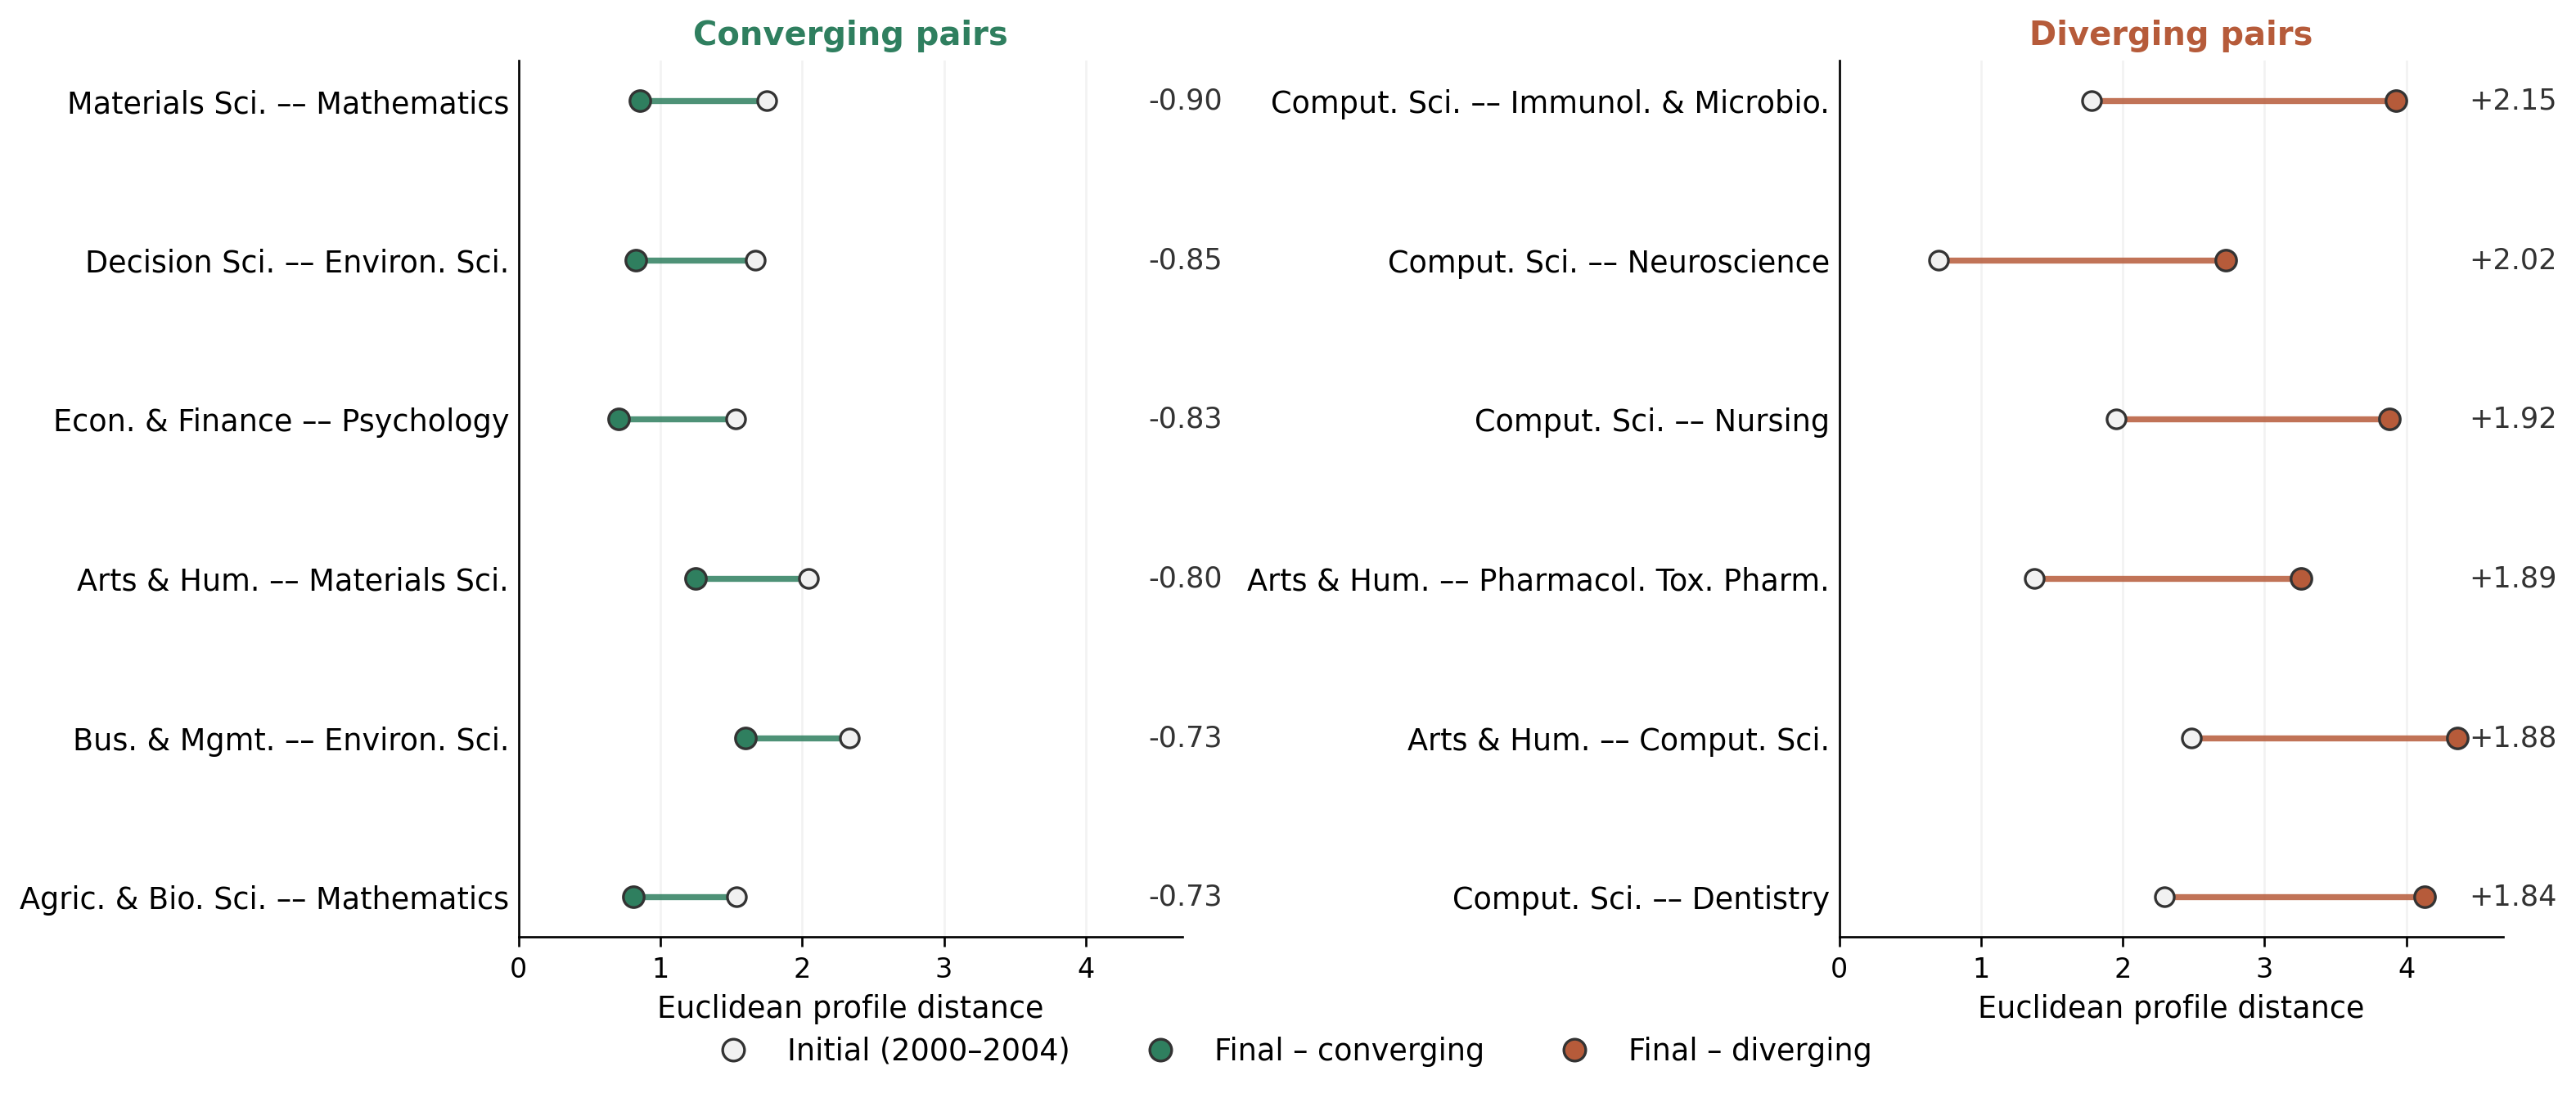
\includegraphics[width=\textwidth]{figures/fig_08_field_convergence_divergence_pairs.png}
\end{figure}

\begin{table}[H]
\centering
\caption[Field convergence and divergence drivers]{Selected field-level convergence and divergence cases}
\label{tab:field_convergence_drivers}
\scriptsize
\begingroup
\setlength{\tabcolsep}{2.5pt}
\begin{tabular}{@{}>{\raggedright\arraybackslash}p{0.27\textwidth} >{\raggedright\arraybackslash}p{0.14\textwidth} >{\raggedleft\arraybackslash}p{0.10\textwidth} >{\raggedright\arraybackslash}p{0.39\textwidth}@{}}
\hline
\textbf{Pair} & \textbf{Relation} & \textbf{$\Delta$ dist.} & \textbf{Largest profile movements} \\
\hline
Materials Sci. -- Mathematics & Converges & -0.90 & Materials Sci.: kNN median -1.5, PCA entropy -1.2; Mathematics: centroid IQR -0.74, PCA entropy -0.73 \\
Decision Sci. -- Environmental Sci. & Converges & -0.85 & Decision Sci.: PCA entropy -1.1, PCA D80 -1.1; Environmental Sci.: kNN median -1.5, PCA D80 -1.2 \\
Economics \& Finance -- Psychology & Converges & -0.83 & Economics \& Finance: PCA D80 -1.2, kNN median -1.1; Psychology: PCA D80 -1.2, PCA entropy -0.99 \\
Computer Sci. -- Immunol. \& Microbio. & Diverges & +2.15 & Computer Sci.: PCA D80 -1.8, PCA entropy -1.5; Immunol. \& Microbio.: kNN median -1.5, kNN CV +1.3 \\
Computer Sci. -- Neuroscience & Diverges & +2.02 & Computer Sci.: PCA D80 -1.8, PCA entropy -1.5; Neuroscience: kNN median -0.97, PCA entropy -0.9 \\
Computer Sci. -- Nursing & Diverges & +1.92 & Computer Sci.: PCA D80 -1.8, PCA entropy -1.5; Nursing: kNN median -1.4, PCA entropy -0.99 \\
\hline
\end{tabular}
\endgroup
\par\vspace{0.15cm}
\footnotesize\textit{Note.} Distances are Euclidean distances between robust-scaled field profiles in the eight windowed structural metrics. Negative final-minus-initial distance indicates convergence; positive values indicate divergence.
\end{table}


The diverging side has a clearer protagonist. Computer Science appears in nine of the ten largest field-level Euclidean divergences, including divergences from Immunology and Microbiology, Neuroscience, Nursing, Dentistry, Energy, and Arts and Humanities. This does not mean that Computer Science becomes semantically remote in topic space; its windowed morphology changes in a way that separates its standardized structural profile from many other fields.

\section{Nearest Neighbors, Bridges, and Isolates}

Nearest-neighbor relations make the matrix interpretable without turning this chapter into a typology. Some neighbors are expected: Chemistry and Materials Science are close, and Nursing and Veterinary are each other's nearest field-level neighbors among the more isolated Health Sciences fields. Other neighbors cross domains: Medicine is nearest to Biochemistry, Genetics and Molecular Biology; Psychology is nearest to Neuroscience; and Energy is nearest to Immunology and Microbiology.

These are bridges only in a morphological sense. They indicate similar profile shape, not collaboration or topical overlap. The strongest static isolates are equally important. Computer Science has the largest nearest-neighbor distance among fields: even its closest field-level neighbor, Physics and Astronomy, remains at distance \(2.75\). It also appears in the farthest static pairs, especially against Pharmacology, Toxicology and Pharmaceutics, Dentistry, Chemistry, Arts and Humanities, and Veterinary.

At subfield level, the same relational logic becomes more extreme. Ecology and Materials Chemistry are the closest static subfield pair, followed by Nutrition and Dietetics with Pulmonary and Respiratory Medicine. The strongest temporal subfield convergence is concentrated around Philosophy, which appears in all ten top Euclidean convergence pairs; the strongest divergence is concentrated around Molecular Medicine, which appears in all ten top Euclidean divergence pairs. These cases show that the most dramatic relational movements occur below the broad field level.

Morphological similarity is a structural comparison under a specific representation. A low distance means that two aggregate metric profiles are close after robust scaling; a high distance means that their profiles differ on one or more metric dimensions. The value of the chapter is relational and descriptive: it shows which scientific regions resemble, approach, or separate from one another in morphological profile space, providing groundwork for Chapter~9.

\paragraph{What this result means.}
Morphological similarity only partly follows taxonomy. Many fields are closest in shape to fields outside their own domain. This does not mean those fields study the same topics; it means their embedded paper distributions are arranged in similar ways. Shape and taxonomic membership are related, but not the same.
